% Exact LaTeX recreation of the supplied Phase-1.pdf
% Compile with pdfLaTeX. Place member pictures in the same folder if required.

\documentclass[11pt,a4paper]{article}

\usepackage[a4paper,left=2.0cm,right=2.0cm,top=1.55cm,bottom=1.55cm]{geometry}
\usepackage[T1]{fontenc}
\usepackage{lmodern}
\usepackage{graphicx}
\usepackage{xcolor}
\usepackage{array}
\usepackage{tabularx}
\usepackage{ragged2e}
\usepackage{enumitem}
\usepackage{fancyhdr}
\usepackage{tikz}
\usepackage{setspace}

% -------------------------------------------------
% COLOURS
% -------------------------------------------------
\definecolor{TitleBlue}{RGB}{61,103,154}

% -------------------------------------------------
% GENERAL SETTINGS
% -------------------------------------------------
\setlength{\parindent}{0pt}
\setlength{\parskip}{0pt}
\renewcommand{\arraystretch}{1.0}

% The supplied document uses a clean sans-serif heading style
% and italic serif-style explanatory text.
\newcommand{\blueheading}[1]{%
    {\sffamily\color{TitleBlue}\fontsize{15}{18}\selectfont #1}%
}

\newcommand{\bluebigheading}[1]{%
    {\sffamily\bfseries\color{TitleBlue}\fontsize{16}{19}\selectfont #1}%
}

\newcommand{\instruction}[1]{%
    {\itshape\fontsize{10.5}{12.5}\selectfont #1}%
}

\newcommand{\answerbox}[2][3.0cm]{%
    \vspace{2pt}
    \noindent
    \fbox{%
        \begin{minipage}[t][#1][t]{\dimexpr\textwidth-2\fboxsep-2\fboxrule\relax}
            \vspace{1mm}
            \itshape #2
        \end{minipage}
    }
}

% -------------------------------------------------
% HEADER / FOOTER
% -------------------------------------------------
\pagestyle{fancy}
\fancyhf{}
\renewcommand{\headrulewidth}{0pt}
\renewcommand{\footrulewidth}{0pt}

\fancyhead[L]{%
    \sffamily\bfseries\itshape\fontsize{10.5}{12}\selectfont
    DSCPP-III-2026-T019
}
\fancyhead[R]{%
    \sffamily\bfseries\fontsize{10.5}{12}\selectfont
    PROJECT PROPOSAL
}
\fancyfoot[R]{%
    \itshape\fontsize{10}{12}\selectfont
    Page \thepage
}
\setlength{\headheight}{14pt}
\setlength{\headsep}{23pt}
\setlength{\footskip}{24pt}

% -------------------------------------------------
% PAGE 1
% -------------------------------------------------
\begin{document}

\vspace*{4mm}

\bluebigheading{PROJECT AND TEAM INFORMATION}

\vspace{8mm}

\blueheading{Project Title}

\vspace{1mm}

\answerbox[0.7cm]{Automated Timetable Clash Detector and Resolver}

\vspace{5mm}

\blueheading{Student / Team Information}

\vspace{2mm}

% Team information table
% Compact 4-member layout so all members remain on Page 1.
\noindent
\begin{tabularx}{\textwidth}{|>{\RaggedRight\arraybackslash}p{0.60\textwidth}|>{\RaggedRight\arraybackslash}X|}
\hline
\begin{minipage}[t]{\linewidth}
\vspace{1.5mm}
\textit{Team Name:}\\[-1mm]
\textit{Team \#}
\vspace{1.5mm}
\end{minipage}
&
\begin{minipage}[t]{\linewidth}
\vspace{1.5mm}
\textit{K2S2}

\textit{DSCPP-III-2026-T019}
\vspace{1.5mm}
\end{minipage}
\\
\hline
\begin{minipage}[t][4.5cm][t]{\linewidth}
\vspace{1.5mm}
\textbf{Team member 1 (Team Lead)}\\[-1mm]
\textit{(Last Name, name: student ID: email, picture):}
\vspace{2.0cm}
\end{minipage}
&
\begin{minipage}[t][3.25cm][t]{\linewidth}
\vspace{1.5mm}
\textit{Singh Pujara, Krish -- 2510010141}\\
\textit{pujarakrish4@gmail.com}

\vspace{2mm}
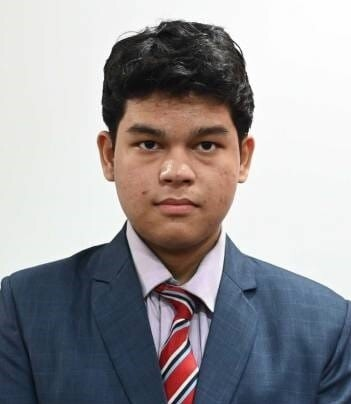
\includegraphics[width=6cm,height=3cm,keepaspectratio]{krish.jpeg}
\end{minipage}
\\
\hline
\begin{minipage}[t][4.5cm][t]{\linewidth}
\vspace{1.5mm}
\textbf{Team member 2}\\[-1mm]
\textit{(Last Name, name: student ID: email, picture):}
\vspace{2.0cm}
\end{minipage}
&
\begin{minipage}[t][3.25cm][t]{\linewidth}
\vspace{1.5mm}
\textit{Bhatt, Kanak -- 2510011122}\\
\textit{theknkbhatt@gmail.com}

\vspace{2mm}
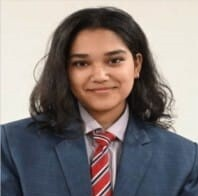
\includegraphics[width=6cm,height=3cm,keepaspectratio]{kanak.jpeg}
\end{minipage}
\\
\hline
\begin{minipage}[t][4.5cm][t]{\linewidth}
\vspace{1.5mm}
\textbf{Team member 3}\\[-1mm]
\textit{(Last Name, name: student ID: email, picture):}
\vspace{2.0cm}
\end{minipage}
&
\begin{minipage}[t][3.25cm][t]{\linewidth}
\vspace{1.5mm}
\textit{Gupta, Sanchit -- 2510010543}\\
\textit{sanchitg2006@gmail.com}

\vspace{2mm}
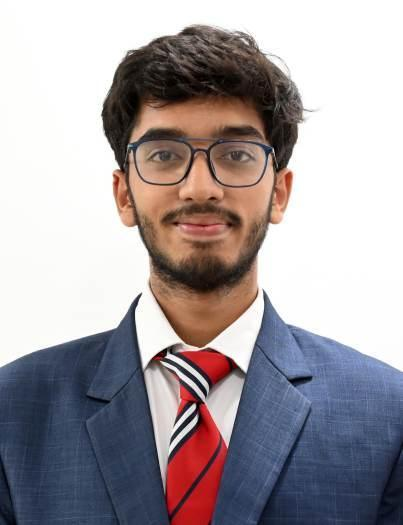
\includegraphics[width=6cm,height=3cm,keepaspectratio]{sanchit.jpeg}
\end{minipage}
\\
\hline
\begin{minipage}[t][4.5cm][t]{\linewidth}
\vspace{1.5mm}
\textbf{Team member 4}\\[-1mm]
\textit{(Last Name, name: student ID: email, picture):}
\vspace{2.0cm}
\end{minipage}
&
\begin{minipage}[t][3.25cm][t]{\linewidth}
\vspace{1.5mm}
\textit{Raturi, Sara -- 2510012612}\\
\textit{sararaturi05@gmail.com}

\vspace{2mm}
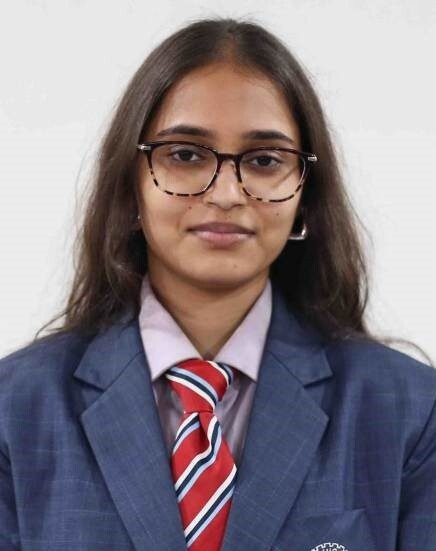
\includegraphics[width=6cm,height=3cm,keepaspectratio]{sara.jpeg}
\end{minipage}
\\
\hline
\end{tabularx}

\newpage

% -------------------------------------------------
% PAGE 2
% -------------------------------------------------

\bluebigheading{PROPOSAL DESCRIPTION (10 pts)}

\vspace{6mm}

\blueheading{Motivation}

\vspace{3mm}

\answerbox[11.1 cm]{Educational institutions face difficulty when they try to organize college timetables. Many administrators do it manually or make use of spreadsheets to manage college timetabling. When the number of student groups and teachers increases every year, the rules for choosing a room or a time slot becomes challenging.

The consequences of manual scheduling are faced by students every day. Clashes in college timetables are often found after the schedule is already released for the public. Students wait outside a room that is already full because two classes were put in the same place. Teachers feel stress because they are given two different student groups at the same hour. It has been observed that fixing these mistakes causes many more problems in other parts of the schedule. Last-minute changes are made by the staff when this confusion happens.

Simple software is used by institutions to help with the work. These programs do not look for mistakes or stop two classes from happening at once. Many people believe that computer tools should do more than just make a list. The working position of fixing every mistake is left to the administrator because the computer does not help with a solution. Because the human must fix the errors, the value of the computer is lost. The burden of actually fixing the problem is left entirely to the administrator, defeating much of the purpose of automation in the first place.

A system that finds mistakes and fixes them provides a great chance for improvement. Success in college timetabling is reached when the system works without human help. This project allows students to use Data Structures and Algorithms alongside C++ ideas in a real situation. It has been stated that using graphs and sorting makes the software very strong. Providing this software is useful because the educational institution needs a better way to work. College timetabling becomes easy when greedy algorithms are applied to the problem. This makes it both practically useful and academically meaningful.
  }

\vspace{7mm}

\blueheading{State of the Art / Current solution}

\vspace{1mm}

\answerbox[6.4 cm]{
Colleges manage timetable creation manually or simply by using grid tools like spreadsheets. Management personnel construct these schedules by hand because they must examine every detail for a conflict. Manual scheduling is frequently found to be error-prone when the quantity of classes and teaching professionals increases each semester.

Different colleges utilize generic timetable creation software which produces a schedule when specific constraints are provided. These systems are not only expensive but they also do not explain how a conflict is identified because the software logic is hidden from the user. While the conflict is flagged, the decision for the fix is not provided by the software. This situation requires the management personnel to perform manual labour to fix the schedule.

This project addresses the gap because DSA techniques are used instead of hidden logic. A clear solution is provided by this project so that timetable creation becomes easier for the college. Many people believe that a transparent approach is better for resolving the conflict because the logic remains visible to everyone.

}

\vspace{70mm}

\blueheading{Project Goals and Milestones }

\vspace{1mm}

\answerbox[9.0cm]{
The main goal of this project is to create a system that automatically finds timetable conflicts. Like rooms, teachers and sections overlapping. And fixes them in a way with as little trouble as possible. This system will replace the slow and mistake-prone way of making timetables by hand. Another goal is to use Data Structures and C++ ideas. Sorting, hashing, graphs and greedy algorithms. To solve a real problem instead of just working on theory.

Milestones

1.	Requirement Analysis & Data Modeling : Decide what information is needed for each class time and create the C++ classes or structures to represent times, rooms, teachers and sections.

2.	Clash Detection : Sort the times by when they happen and build the sweep-line algorithm to find overlapping bookings for rooms, teachers and sections.

3.	Fast Lookup & Schedule Storage : Make a way to quickly check availability using hash tables and store the schedule for each room.

4.	Conflict Graph & Resolution Engine : Create a conflict graph from the clashes found use DFS or BFS to find groups of conflicts and use graph coloring to assign new time slots.

5.	Auto-Resolution Logic : Add a way to fix conflicts that graph coloring can’t handle directly by using priorities and searching for the available time slot.

6.	Testing & Output : Test the system, with sizes of sample data check that the detection and fixing work properly and finish how the results are shown. A list of conflicts and the final timetable.
}

\vspace{8mm}

\blueheading{Project Approach}

\vspace{1mm}

\answerbox[8.0 cm]{1. Input and Data Modeling: Timetable data (subject, faculty, room, section, day, time) is stored in arrays/vectors and represented using C++ classes/structures

2. Preprocessing: All class sessions are sorted using a manually implemented sorting techniques (Merge Sort or Quick Sort)

3. Clash Detection: A sweep-line technique scans through the sorted sessions and checks for nearby overlapping intervals for shared room, faculty, or section. The priority is to achieve O(n log n) performance instead of a slow O(n²)

4. Fast Lookup: Hash tables are used to instantly check room/faculty/section availability at any given time slot.

5. Conflict Modeling: Detected clashes are represented as a graph, where each clashing session is a node and edges represent conflicts between them. DFS/BFS is used to identify fully connected conflict groups.

6. Resolution: A greedy graph coloring algorithm assigns time slots to each session. A priority-based greedy algorithm (core subjects/senior faculty prioritized) shifts the least disruptive session to the nearest available slot if no valid free slots are available. 

7. Output: The final clash-free timetable is displayed along with a list of resolved conflicts. }

\newpage

% -------------------------------------------------
% PAGE 3
% -------------------------------------------------

\blueheading{System Architecture (High Level Diagram)}

\vspace{5mm}

{
    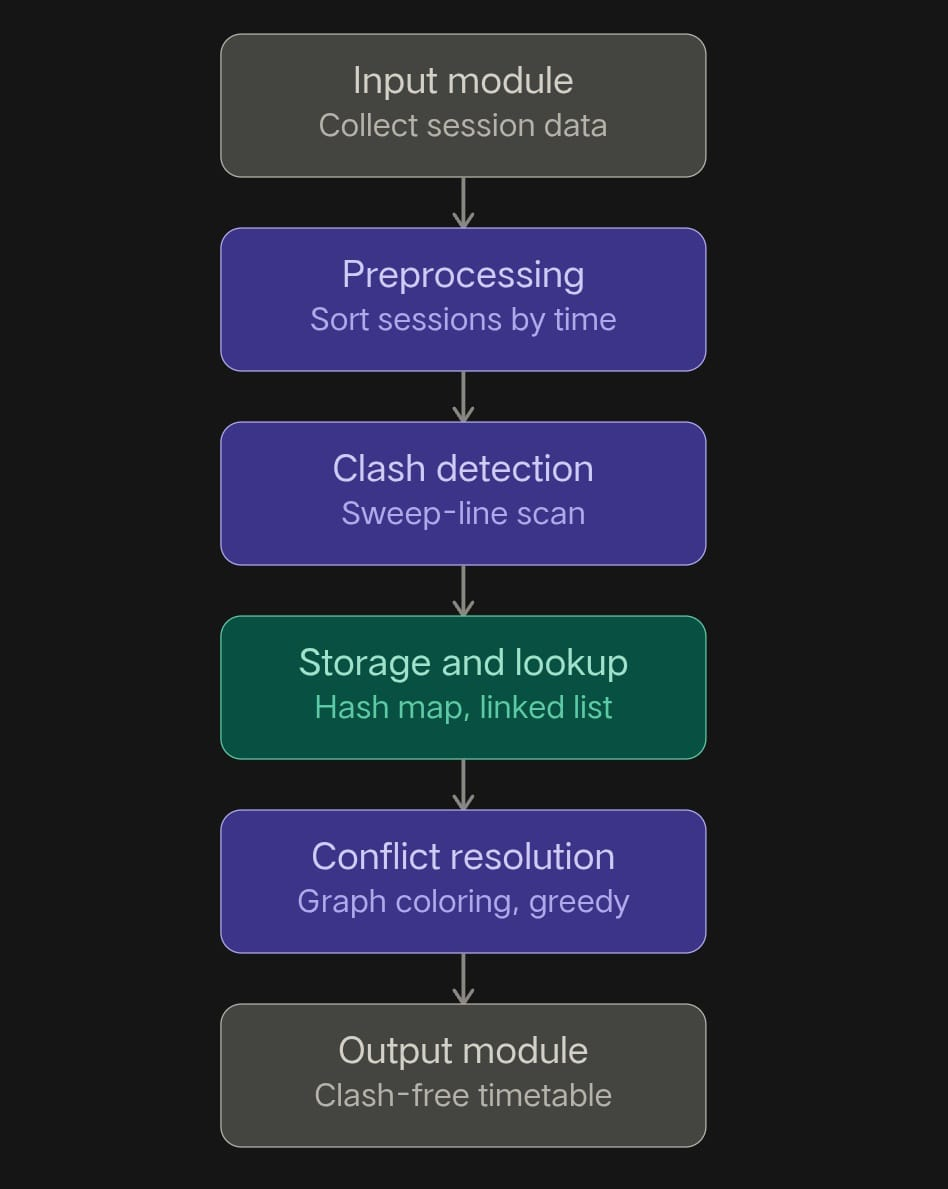
\includegraphics[width=8cm]{diagram.jpeg}
}

\vspace{11mm}

\blueheading{Project Outcome / Deliverables }

\vspace{1mm}

\answerbox[6 cm]{ 1. This system is built using C++ language and it is capable of taking a dataset as input, performs manipulations and identifies room, faculty and section conflicts

2. It mainly uses graph colouring and greedy algorithms to detect the clashes and provides conflict free slots, instead of just flagging errors for manual fixing.

3. A report is generated as the output which shows the list of clashes along with the original and final resolved timetable.

4. Handles large data through sorting and using hashing-based lookups.

5. A working demonstration on sample datasets of varying sizes, showing correctness and performance of the detection and resolution logic.

6. An extensible codebase that can later be built upon for a full timetable generation tool, rather than just conflict-checking.}

\vspace{10mm}

\blueheading{Assumptions}

\answerbox[3.5cm]{1. The input data (subject, professor, room, section, time period) is well-organized without any kind of repetition or incorrect data.

2. Each lecture in a classroom lasts for a certain amount of time.

3. Priorities (like solving conflicts automatically, where, for example, core courses will be prioritized over electives) are fixed and predetermined.

4. Only one campus is assumed to exist and there will be no inter-campus scheduling involved.

5. There are sufficient number of time periods available for solving conflicts.}

\vspace{20mm}

\blueheading{References}

\vspace{1mm}

\answerbox[1.8cm]{1. GeeksForGeeks - To understand DSA and C++ concepts

2. W3Schools– For better understanding deeper concepts of C++, classes, objects etc.

3. Book- ’Data Structures using C by Reema Thareja’ for concepts of Arrays and Linked List.}

\end{document}
